\chapter{Related Work} \label{chap:csr}

This section considers some existing frameworks and compares them to our solution approach. 
We will only consider major features and neglect minor technical differences and implementation details. 
We will focus on the topics like \texttt{UI Prototyping}, \texttt{Task Based Usability Tasting}, \texttt{Continuous Experiments}, and \texttt{Model-based} approaches. 

\section{State of the Art Research}

\paragraph{Model-Based UIs:}
Various modeling languages are introduced for formalizing the User Interface (UI).
A standardized modeling language for software product content, abstract UI model, user interactions, and control behavior is Interaction Flow Modeling Language (IFML) \cite{article:ifml:piero}. 
As a result, IFML focuses on the platform-independent display of the user interface that is transferable between many platforms and devices.
Cameleon \cite{article:cameleon:balme} is a framework that divides the user interface into several elements to maximize the parts' reusability in various user, platform, and environment situations.
A platform-independent abstract UI, a platform-dependent concrete UI, and a device-dependent final UI are the layers the framework offers to accomplish this.

\paragraph{Continuous Experimentation:}
The idea of continuously testing the software product's fundamental assumptions on the users is through continuous experimenting.
Several conceptual models and platform designs have been suggested to support the process.
A feature with a high priority is chosen and added to the product using Hypothesis Experiment Data-Driven Development (HYPEX) \cite{article:hypex:model}, creating a feature backlog from strategic product goals.
Another research is Rapid Iterative value creation Gained through High-frequency Testing (RIGHT) \cite{article:right:model} that is very similar to HYPEX is used to identify the hypotheses developed from the models.
These hypotheses are tested using experimentation, and the best feature is implemented in the product.
In contrast to HYPEX and RIGHT, Qualitative/quantitative Customer-driven Development (QCD) \cite{article:qq:helena} focuses on combining the qualitative customer feedbacks with the quantitative customer observations.  

However, none of the conceptual models and the continuous experiments focus on integrating the models in the experimentation of the UI prototypes.
Therefore, we plan to develop a tool that combines all the above requirements.
Figure \ref{relatedwork:img:comparative} does a comparative analysis of the existing tools and our proposed tool.
% \paragraph{Task-based Usability Testing} There is much evidence showing that task-based usability testing has improved the usability of the UI \cite{article:tbup:frank, article:tbup:kari}.
\section{Comparison of Tools based on Requirements}
This section compares the tools for UI prototyping based on the requirements;\\ \texttt{(1) Model-Based} approach, \texttt{(2) Continuous Experimentation}, and \\ \texttt{(3) Task-based Usability testing}.

\paragraph{UI Prototyping tools:} The current popular platform for UI Prototyping are Figma\footnote{Figma: \url{https://www.figma.com/}}, InVision Studio\footnote{InVision Studio: \url{https://www.invisionapp.com/}}, and Adobe XD\footnote{AdobeXD: \url{https://www.adobe.com/products/xd.html}}.
With a browser-based, cloud-hosted platform, Figma is a tool that facilitates collaboration and accessibility for UI/UX designers, developers, and anybody else on a team.
Figma integrates various plugins like Autoflow for illustrating user flows and Figmotion for creating animations, enhancing its usability \cite{article:comparative:prototypes}.
Similarly, InVision Studio allows designers to quickly build functional prototypes and share them with others with many well-designed tools.
A vector-based method for building prototypes is available via Adobe XD, along with tools for adding interactions, transitions, and other dynamic features \cite{article:comparative:prototypes}.
Because of its vector-based property, scaling and resizing the elements is done efficiently.

\begin{figure}[ht]
    \centering
    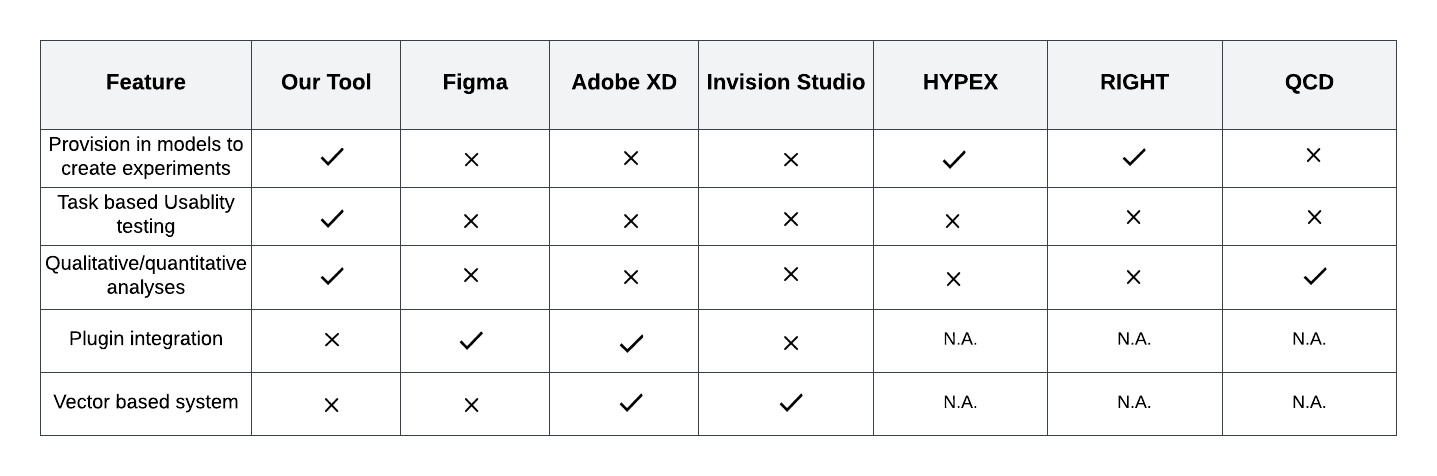
\includegraphics[scale=0.28]{images/related-work/Comparative.png}
    \caption{Comparative study for different tools}
    \label{relatedwork:img:comparative}
\end{figure}
